\textbf{Pour cette première partie, aucune justification n'est demandée et une seule réponse est possible par question. Pour chaque question, reportez son numéro sur votre copie et indiquez votre réponse.}

	Une réponse fausse ou l'absence de réponse n'enlève aucun point.

\bigskip

	\textbf{Question 1}

On veut comparer deux nombres réels notés $A$ et $B$.

On sait que la différence $A - B$ est strictement positive. Alors :

\begin{multicols}{4}
\begin{enumerate}[label=\textbf{\alph* .}]
\item $A<B$
\item $A>B$
\item $A=B$
\item On ne peut pas savoir
\end{enumerate}
\end{multicols}

	\textbf{Question 2}

On considère le nombre $C=\dfrac{1}{2}+3\times\dfrac{5}{6}$. On a :

\begin{multicols}{4}
\begin{enumerate}[label=\textbf{\alph* .}]
\item $C = 2$
\item $C = \dfrac{35}{12}$
\item $C = \dfrac{35}{2}$
\item $C = 3$
\end{enumerate}
\end{multicols}

\textbf{Question 3}

On considère le nombre $D=3 \times 2^5 \times 2^3$. On a :

\begin{multicols}{4}
\begin{enumerate}[label=\textbf{\alph* .}]
\item $D = 3\times 2^{8}$
\item $C = 6^{8}$
\item $C = 3\times 2^{15}$
\item $C = 7^{8}$
\end{enumerate}
\end{multicols}


\textbf{Question 4}

On considère le nombre $E = \np{999} \times \np{1001}$. Un ordre de grandeur de $E$ est :

\begin{multicols}{4}
\begin{enumerate}[label=\textbf{\alph* .}]
\item $\np{1000}$
\item $\np{10000}$
\item $\np{100000}$
\item $\np{1000000}$
\end{enumerate}
\end{multicols}

\textbf{Question 5}

Quand on développe $(x+2)^2$, on obtient :

\begin{multicols}{4}
\begin{enumerate}[label=\textbf{\alph* .}]
\item $x^2+4x+4$
\item $2x+4$
\item $x^2+4$
\item $x^2-4$
\end{enumerate}
\end{multicols}

\textbf{Question 6}

L'équation $ 3x - 5 = x + 3 $ a pour solution :

\begin{multicols}{4}
\begin{enumerate}[label=\textbf{\alph* .}]
\item $ x = -4 $
\item $ x = 8 $
\item $ x = 6 $
\item $ x = 4 $
\end{enumerate}
\end{multicols}

\pagebreak

\textbf{Question 7}

Dans une boîte de 60 chocolats 40~\% sont des chocolats au lait. Combien y a-t-il de chocolats au lait dans la boite ?

\begin{multicols}{4}
\begin{enumerate}[label=\textbf{\alph* .}]
\item 20
\item 24
\item 25
\item 40
\end{enumerate}
\end{multicols}

\textbf{Question 8}

Le taux d'évolution équivalent à une baisse de 10~\% suivie d'une baisse de  20~\% est :

\begin{multicols}{4}
\begin{enumerate}[label=\textbf{\alph* .}]
\item $-38~\%$
\item $-30~\%$
\item $-28~\%$
\item $-18~\%$
\end{enumerate}
\end{multicols}

\textbf{Question 9}

\begin{minipage}{0.5\linewidth}
	Une droite est représentée ci-contre. L'équation réduite de cette droite est :\\
	
\begin{enumerate}[label=\textbf{\alph* .}]
\item $y = -2x +3 $
\item $y = 3x + \np{1.5} $
\item $y = \np{-0.5}x + \np{3} $
\item $y = \np{-2}x + \np{1.5} $
\end{enumerate}


	\end{minipage}
	\hfill
	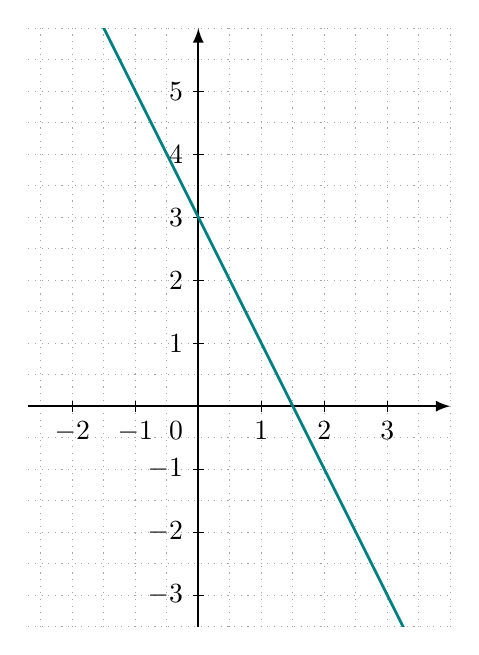
\begin{tikzpicture}[x = 8mm, y = 8mm, baseline={(current bounding box.center)}]
		\draw[gray!70, xstep=0.5,ystep=0.5,dotted] (-2.7,-3.5) grid (4,6);
		\clip (-2.7,-3.5) rectangle (4,6);
		\draw[thick,-latex] (-2.7,0)--(4,0);
		\draw[thick,-latex] (0,-3.5)--(0,6);
		\foreach \x in {-2,-1,1,2,3}{
			\draw (\x,2pt)--(\x,-2pt) node[below]{$\x$};}
		\foreach \y in {-3,-2,-1,1,2,...,5}{
			\draw (2pt,\y)--(-2pt,\y) node[left]{$\y$};}
		\node[below left] (O) at(-2pt,-2pt) {0};
		\draw[teal,line width=1pt] plot[domain=-2:4] (\x,{-2*\x+3}) ;
	
	\end{tikzpicture}\hfill~











\textbf{Question 10}
	
	En physique, l'énergie cinétique d'un véhicule est donnée par la formule :
	\[E=\dfrac{1}{2}m v^{2}\]
	où $m$ représente la masse du véhicule et $v$ sa vitesse.
	
	On souhaite exprimer $v$ en fonction de $E$ et $m$. Une expression de $v$ est :
	
\begin{multicols}{4}
\begin{enumerate}[label=\textbf{\alph* .}]
	\item $v=\sqrt{\dfrac{2E}{m}}$
	\item $v=\dfrac{2E}{m}$ 
	\item $v=\sqrt{E-\dfrac{1}{2}m}$ 
	\item $v=\sqrt{2mE}$ 
\end{enumerate}
\end{multicols}


		\textbf{Question 11}

	\begin{minipage}{0.52\linewidth}		
		Une fonction $h$ définie sur $[-3~;~4]$ est représentée ci-contre.
		
		L'équation $h(x)=2$ a pour ensemble solution :
		
		\begin{enumerate}[label=\textbf{\alph* .}]
			\item $\mathcal{S}=\{2\}$
			\item $\mathcal{S}=\{-2~;~2~;~3\}$
			\item $\mathcal{S}=[-2~;~3]$
			\item $\mathcal{S}=\{-0,5~;~0,5\}$
		\end{enumerate}
	\end{minipage}
	\hfill
	\begin{minipage}{0.42\linewidth}
		\centering
		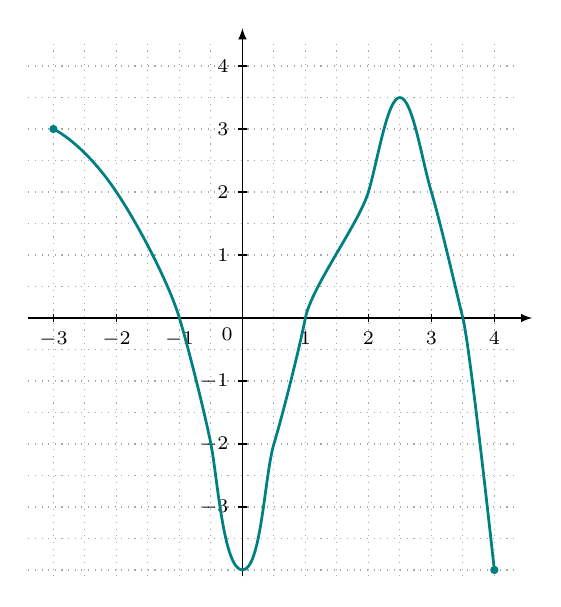
\begin{tikzpicture}[x=8mm,y=8mm,baseline={(current bounding box.center)}]
			\draw[gray!70,dotted] (-3.4,-4.1) grid[step=0.5] (4.4,4.4);
			\draw[-latex] (-3.4,0)--(4.6,0);
			\draw[-latex] (0,-4.1)--(0,4.6);
			\foreach \x in {-3,-2,-1,1,2,3,4}{\draw (\x,1.5pt)--(\x,-1.5pt) node[below,font=\scriptsize]{$\x$};}
			\foreach \y in {-3,-2,-1,1,2,3,4}{\draw (1.5pt,\y)--(-1.5pt,\y) node[left,font=\scriptsize]{$\y$};}
			\node[below left,font=\scriptsize] at (0,0) {0};
			\draw[teal,line width=1pt]
				(-3,3) node (A) {} .. controls ++(0.2,-0.1) and ++(-0.4,0.6) ..
				(-2,2) .. controls ++(0.4,-0.6) and ++(-0.15,0.5) ..
				(-1,0) .. controls ++(0.15,-0.5) and ++(-0.1,0.5) ..
				(-0.5,-2) .. controls ++(0.1,-0.5) and ++(-0.3,0) ..
				(0,-4) .. controls ++(0.3,0) and ++(-0.15,-0.5) ..
				(0.5,-2) .. controls ++(0.15,0.5) and ++(-0.1,-0.5) ..
				(1,0) .. controls ++(0.1,0.5) and ++(-0.15,-0.5) ..
				(2,2) .. controls ++(0.15,0.5) and ++(-0.2,0) ..
				(2.5,3.5) .. controls ++(0.2,0) and ++(-0.15,0.5) ..
				(3,2) .. controls ++(0.15,-0.5) and ++(-0.1,0.4) ..
				(3.5,0) .. controls ++(0.1,-0.4) and ++(-0.1,0.9) ..								
				(4,-4) node (B) {}
				;
			\fill[teal] (A) circle (1.5pt)  (B) circle (1.5pt);					
		\end{tikzpicture}
	\end{minipage}

\textbf{Question 12}
	
	Un élève a obtenu une série de trois notes 9~; 11~; 13 en mathématiques. Il a déterminé la moyenne et la médiane de cette série.
	
	Il a obtenu deux nouvelles notes : 10 et 17 et obtient ainsi une nouvelle série de notes : 9~; 10~; 11~; 13~; 17.
	
	Laquelle des quatre propositions est vraie ?
	
	\begin{enumerate}[label=\textbf{\alph* .}]
	\item Les moyennes des deux séries sont égales et les médianes sont égales.
	\item Les moyennes des deux séries sont égales et les médianes sont différentes.
	\item Les moyennes des deux séries sont différentes et les médianes sont égales.
	\item Les moyennes des deux séries sont différentes et les médianes sont différentes.
	\end{enumerate}
